\documentclass[12pt]{article}
\usepackage[onehalfspacing]{setspace}
\usepackage{dcolumn}
\usepackage[left=1in, top=1in, bottom=1in]{geometry}
\usepackage{graphicx}
\usepackage[table,xcdraw]{xcolor}
\usepackage{longtable}
\usepackage{float}
\usepackage{listings}
\usepackage{xcolor}
\usepackage{amsmath}
\usepackage{amsfonts}
\usepackage{amssymb}


\lstset{language=R,
    basicstyle=\small\ttfamily,
    stringstyle=\color{commentgreen},
    otherkeywords={0,1,2,3,4,5,6,7,8,9},
    morekeywords={TRUE,FALSE},
    deletekeywords={data,frame,length,as,character},
    keywordstyle=\color{blue},
    commentstyle=\color{commentgreen},
}
\begin{document}

\title{Syndicate 5 Statistical Learning Problem Set \#2}
\maketitle
{\setlength{\parindent}{0cm}

\section*{Fishing Mode}
\subsection*{Ordered Logit Model}
An initial review of the data set identified that the price of beach and pier were identical. This was further highlighted in the correlation matrix (Appendix Table 3) where beach and pier price had a correlation of 1, as such, the beach price was excluded from the model. The boat and charter price and catch rate also had a strong correlation at 0.9963 and 0.9364, respectively. However, as the variables were not perfectly correlated, these predictors were retained.\\


The ordered logit model was then constructed with mode of fishing as the outcome and price and catch rate as predictors, using the prescribed order of Beach $<$ Pier $<$ Boat $<$ Charter. The following results were obtained - refer to Appendix Table 1 for details.\\

$$y_i = \begin{cases}
1(Beach) & \text{if} \: z_i < 0.6893\\
2(Pier) & \text{if} \: 0.6893 \leq z_i < 2.0414\\
3(Boat) & \text{if} \: 2.0414 \leq z_i < 3.9392\\
4(Charter) & \text{if} \: z_i \geq 3.9392
\end{cases}$$

$z_i = 0.0059Price.Pier_i - 0.1246Price.Boat_i + 0.1153Price.Charter_i + 0.6535Catch.Beach_i - 4.0614Catch.Pier_i + 0.9066Catch.Boat_i + 0.1986Catch.Charter_i + \varepsilon_i$\\
$\varepsilon_i \sim Logistic(\mu = 0, s = 1)$\\

The results identified that the pier/beach and charter price increased the propensity for an individual to choose a charter. In contrast, the boat price decreased the propensity to choose a charter. All price predictors were statistically significant to a 0.01 level. These results were counter-intuitive as an increase in charter price should intuitively reduce the propensity of a customer choosing a charter. This may point to a multicollinearity issue stemming from a strong correlation between boat and charter price. Examining the odds ratio plots in Appendix Figure 2, the odds ratios against pier/beach price odds shows a general upward trend, emphasising the positive relationship between pier/beach price and the propensity to choose a ‘higher’ mode of fishing at each interval. The opposite relationship is shown against boat price odds where a general downward trend is illustrated, highlighting that boat price is associated with a decrease in propensity to choose a charter at all mode intervals. Oddly, the charter price plots show a general downward trend which does not align with the sign of the estimated coefficient. Thus, further emphasizing potential multicollinearity.\\

Looking at the catch rate, the pier catch rate was the only statistically significant predictor (to a significance level of 0.01). The pier catch rate had a negative relationship with the propensity to choose a charter. Again, these results were unexpected as the boat or charter catch rate should intuitively have an influence on the mode choice. This may also point to a multicollinearity issue as boat and charter catch rates were strongly correlated. Looking at the odds ratio plots shown in Appendix Figure 2 a clear trend is not shown. This may be an indicator that the catch rate does not explain as much of the variance in mode choice compared to price.\\ 


\subsection*{Multinomial Logit Model}
\subsubsection*{Question 1}
In order to facilitate the comparison with the ordered model, we use the same independent variables as the previous model for the unordered multinomial logit model. In this case, beach is used as the as the reference mode. The fit of the model is shown in Appendix Table 2.\\

The following effects are found on the probabilities of the fishing modes:
\begin{itemize}
\item The probability that an individual chooses boat or charter instead of beach \textit{increases} if pier price increases (no real effect on pier vs beach as effect is insignificant at the 5\% level).
\item The probability that an individual chooses boat, charter or pier instead of beach \textit{all decrease} if boat price or the catch rate of pier increases.
\item The probability that an individual chooses boat, charter or pier instead of beach \textit{all increase} if charter price, the catch rate of beach or the catch rate of charter increases. Note that these effects are insignificant at the 5\% level for the case of the charter catch rate increasing.
\item The probability that an individual chooses boat or pier instead of beach \textit{decreases} and the probability that they choose charter instead of beach \textit{increases} if the catch rate of boat increases. However, all of these effects are insignificant at the 5\% level.
\end{itemize}

Additionally, looking at the odds ratios (see Appendix Figure 1) of boat, charter and pier relative to beach tells us that in general, individuals tend to be much more likely to choose boat or charter than the beach as their fishing mode while only slightly more likely to choose the pier over the beach (note that the fourth plot is the third plot on a smaller scale).

\subsubsection*{Question 2}
The fundamental difference is that the choices in the ordered model have an order of agreed superiority while the multinomial model doesn't.\\

In our example, the ordered model assumes that everyone sees "Charter" as the best option, followed by "Boat", "Pier" and "Beach" respectfully. However, choices are influenced by the price and catch rates of each mode. Thus, the higher an individual's utility, the more likely they are to go with a "superior" option. Furthermore, in ordered models, there is no intercept as thresholds are estimated instead, making identification easier. Likelihoods are then allocated based on these thresholds and utilities.\\

For unordered outcomes, no preferences means that we must model probabilities relatively. Parameters are estimated for every group (except one reference group) to tell us the effect of a single change on each group and hence give the utility for each choice from which probabilities are allocated. Notably, there isn't an intercept estimated as thresholds aren't calculated.\\

For this fishing example, the unordered model is likely to be more suitable as individuals are unlikely to rank each mode the same due to personal preferences. This is backed up by the unordered model having a much lower AIC (2,181.346 vs 2673.745).


\section*{Credit Card Balances - Revisited}
\subsection*{Tobit Regression}
Running a Tobit model based on the new variable $BalanceRatio_i$ gives us the model below (see Appendix Table 4 for a detailed side by side with week 1's model).\\

$BalanceRatio_i = -0.1386 -0.002587Income_i + 0.000005766Income^2_i + 0.001159Rating_i - 0.0000006128Rating^2_i - 0.0001993Age_i + 0.1018Student_i$\\

$Income_i$, $Rating_i$, $Age_i$ and $Student_i$ (and by extension, $Income^2_i$ and $Rating^2_i$) are all drivers of credit card utilization since all are statistically significant to the 1\% level, as was the case in week 1. All of the linear terms maintain the same sign, implying the same directional effect on the credit card balance ratio as they had on the credit card balance. Interestingly, the squared terms now both have the opposite sign coefficients as they did in week 1. Now the coefficient on $Income^2_i$ is positive. On the other hand, the coefficient on $Rating^2_i$ is now negative.\\

Neither of these changes contradict the model significantly (coefficients on the squared terms are very small in both models although, still significant) however, there are differences in what dependant variable is. Using a balance ratio means that individuals with low balances but are near their limit (due to a lower limit) now have a relatively high value for the dependant variable while they previously had a low one. This has likely caused some redistribution of our actual and thus, fitted values in our new model.\\

The change in $Income^2_i$ suggests people \emph{get closer to their limits} at a higher rate at higher incomes while in week one the negative sign on $Income^2_i$ suggested people get \emph{larger balances} at a lower rate at higher incomes. The change in $Rating^2_i$ suggests that people \emph{get closer to their limit} at a lower rate with higher ratings while in week one the positive sign on $Rating^2_i$ suggested people get \emph{larger balances} at a higher rate at higher ratings. 

\subsection*{Poisson Regression}
\subsubsection*{Question 1}
A Poisson regression model was constructed to assess how a customer’s demographic characteristics may explain the number of credit cards held. The initial model included all available predictor variables. Each predictor that was not significant was then removed one at a time, starting with the predictor with the highest p-value. Once removed, the AIC of the new model was compared against the previous model to check if it had improved.\\

As described in the model selection table (Appendix Table 6), the final model only included income and rating predictors. Looking at the model coefficients, income had a negative association with the number of credit cards i.e. the higher the income, the lower expected number of credit cards. In contrast, the rating coefficient was positive, indicating as the rating increase, the number of credit cards a customer had also increased.\\

The dispersion parameter was first calculated to assess if the model is underdispersed or overdispersed. The calculated dispersion parameter was $\omega = 0.6268$, indicating that the model may be underdispersed. The following hypothesis test was then run to understand if the variance in the standardised residual terms was equal to 1. The test was as follows:\\
$$H_0: Var(z_i) = 1 \; \; \; \; \; H_1: Var(z_i) < 1$$
$$p-value = 5.9705*10^{-10}$$

The p-value from the hypothesis test was less than a significance level of 0.001 indicating that the null hypothesis should be rejected in favour of the alternate. Hence, the variance of the standardised residual term is less than 1, confirming the model is underdispersed.\\

Since, the model is underdispersed, a quasi-Poisson regression was run using the same predictors. Results from this analysis are detailed in Table 5. In the new quasi model, the predictor coefficients were unchanged, however, the standard error terms decreased, initiating a decrease in the p-values (this is due to the model being previously underdispersed). Based on the new p-values both income and rating were deemed  significant.\\

As an additional check, the quasi model was re-run with predictors from previous models (model 5 and model 4). Age and education predictors were still deemed insignificant. Hence, the initial quasi model with only income and rating predictors was retained as the final recommended model (again, see Appendix Table 5).

\subsubsection*{Question 2}
The linear regression model on $Cards_i$ with the exact same set of independent variables as the previous Poisson regression model is below and in Appendix Table 6.\\
$$Cards_i = 2.6720 - 0.0063Income_i + 0.01605Rating_i$$

Compared with the result of linear regression model has similar coefficients as the Poisson model and all terms are significant. This is because the Poisson regression model returns the coefficient in exponential form. These two models return very similar predictions given by the same test data as long as independent parameters locates in a reasonable range (not too small or large).\\

However, the main difference between simple linear regression model and Poisson model is the initial assumption about the distribution of parameters. In linear regression model, it is assumed that the error term of the model follows the normal distribution, and the Poisson regression model suggest that the dependent variable Y follows the Poisson distribution and could be explained by a linear combination of independent parameters.\\
  
In this case, the dependent variable, $Cards_i$, is discrete and counted, with non-negative values. The Poisson regression model is designed to predict the discrete variables, so it is generally a better fit for this case. Moreover, the linear regression model would return negative values in certain circumstances, which is obviously inconsistent with the actual situation. Therefore, the Poisson regression model is more appropriate in this case.


\section*{Appendix}
\begin{table}[H]
\parbox{.45\linewidth}{
\centering
  \caption{Ordered Logit Model} 
  \label{} 
\resizebox{7cm}{!}{
\begin{tabular}{@{\extracolsep{5pt}}lc} 
\\[-1.8ex]\hline 
\hline \\[-1.8ex] 
 & \multicolumn{1}{c}{\textit{Dependent variable:}} \\ 
\cline{2-2} 
\\[-1.8ex] & mode \\ 
\hline \\[-1.8ex] 
 price.pier & 0.006$^{***}$ \\ 
  & (0.001) \\ 
  & \\ 
 price.boat & $-$0.125$^{***}$ \\ 
  & (0.014) \\ 
  & \\ 
 price.charter & 0.115$^{***}$ \\ 
  & (0.014) \\ 
  & \\ 
 catch.beach & 0.653 \\ 
  & (0.619) \\ 
  & \\ 
 catch.pier & $-$4.061$^{***}$ \\ 
  & (0.756) \\ 
  & \\ 
 catch.boat & 0.907 \\ 
  & (0.928) \\ 
  & \\ 
 catch.charter & 0.199 \\ 
  & (0.266) \\ 
  & \\ 
\hline \\[-1.8ex] 
Observations & 1,182 \\ 
\hline \\[-1.8ex] 
AIC & 2673.745 \\
\hline
\hline \\[-1.8ex] 
\textit{Note:}  & \multicolumn{1}{r}{$^{*}$p$<$0.1; $^{**}$p$<$0.05; $^{***}$p$<$0.01} \\ 
\end{tabular} 
}
}
\hfill
\parbox{.45\linewidth}{
\centering
  \caption{Multinomial Logit Model} 
  \label{} 
\resizebox{8cm}{!}{
\begin{tabular}{@{\extracolsep{5pt}} cccc} 
\\[-1.8ex]\hline 
\hline \\[-1.8ex] 
 & Boat & Charter & Pier \\ 
\hline \\[-1.8ex] 
(Intercept) & $$-$13.429^{***}$ & $$-$16.149^{***}$ & $$-$7.179^{**}$ \\ 
price.pier & $0.032^{***}$ & $0.027^{***}$ & $$-$0.005$ \\ 
price.boat & $$-$0.579^{***}$ & $$-$0.670^{***}$ & $$-$0.321^{***}$ \\ 
price.charter & $0.556^{***}$ & $0.652^{***}$ & $0.320^{***}$ \\ 
catch.beach & $58.579^{***}$ & $60.639^{***}$ & $37.511^{***}$ \\ 
catch.pier & $$-$86.664^{***}$ & $$-$86.885^{***}$ & $$-$51.327^{***}$ \\ 
catch.boat & $$-$0.521$ & $0.368$ & $$-$1.784$ \\ 
catch.charter & $0.306$ & $0.119$ & $0.100$ \\ 
\hline \\[-1.8ex] 
AIC & & 2181.346 \\
\hline
\hline \\[-1.8ex] 
\textit{Note:} & & \multicolumn{2}{r}{$^{*}$p$<$0.1; $^{**}$p$<$0.05; $^{***}$p$<$0.01} \\ 
\end{tabular}
}
}
\end{table}

\begin{table}[!htbp] \centering 
  \caption{Correlation Matrix} 
  \label{} 
\resizebox{15cm}{!}{
\begin{tabular}{@{\extracolsep{5pt}} ccccccccc} 
\\[-1.8ex]\hline 
\hline \\[-1.8ex] 
 & price.beach & price.pier & price.boat & price.charter & catch.beach & catch.pier & catch.boat & catch.charter \\ 
\hline \\[-1.8ex] 
price.beach & $1$ & $1$ & $0.112$ & $0.141$ & $0.332$ & $0.226$ & $$-$0.098$ & $$-$0.027$ \\ 
price.pier & $1$ & $1$ & $0.112$ & $0.141$ & $0.332$ & $0.226$ & $$-$0.098$ & $$-$0.027$ \\ 
price.boat & $0.112$ & $0.112$ & $1$ & $0.996$ & $0.213$ & $0.253$ & $$-$0.041$ & $$-$0.023$ \\ 
price.charter & $0.141$ & $0.141$ & $0.996$ & $1$ & $0.245$ & $0.287$ & $$-$0.063$ & $$-$0.027$ \\ 
catch.beach & $0.332$ & $0.332$ & $0.213$ & $0.245$ & $1$ & $0.818$ & $0.139$ & $0.208$ \\ 
catch.pier & $0.226$ & $0.226$ & $0.253$ & $0.287$ & $0.818$ & $1$ & $0.134$ & $0.187$ \\ 
catch.boat & $$-$0.098$ & $$-$0.098$ & $$-$0.041$ & $$-$0.063$ & $0.139$ & $0.134$ & $1$ & $0.936$ \\ 
catch.charter & $$-$0.027$ & $$-$0.027$ & $$-$0.023$ & $$-$0.027$ & $0.208$ & $0.187$ & $0.936$ & $1$ \\ 
\hline \\[-1.8ex] 
\end{tabular} 
}
\end{table} 


\begin{table}[H]
\parbox{.45\linewidth}{
\centering
  \caption{Week 1 OLS vs Week 5 Tobit} 
  \label{} 
\resizebox{8cm}{!}{
\begin{tabular}{@{\extracolsep{5pt}}lcc} 
\\[-1.8ex]\hline 
\hline \\[-1.8ex] 
 & \multicolumn{2}{c}{\textit{Dependent variable:}} \\ 
\cline{2-3} 
\\[-1.8ex] & Balance & BalanceRatio \\ 
\\[-1.8ex] & (1) & (2)\\ 
\hline \\[-1.8ex] 
 Income & $-$6.238$^{***}$ & $-$0.002587$^{***}$ \\ 
  & (0.486) & (0.00009133) \\ 
  & & \\ 
 I(Income$\hat{\mkern6mu}$2) & $-$0.021$^{***}$ & 0.000005766$^{***}$ \\ 
  & (0.003) & (0.0000006255) \\ 
  & & \\ 
 Rating & 2.471$^{***}$ & 0.001159$^{***}$ \\ 
  & (0.136) & (0.00003103) \\ 
  & & \\ 
 I(Rating$\hat{\mkern6mu}$2) & 0.002$^{***}$ & $-$0.0000006128$^{***}$ \\ 
  & (0.0002) & (0.00000003681) \\ 
  & & \\ 
 Age & $-$0.729$^{***}$ & $-$0.0001993$^{***}$ \\ 
  & (0.261) & (0.00004925) \\ 
  & & \\ 
 StudentYes & 428.341$^{***}$ & 0.1018$^{***}$ \\ 
  & (14.755) & (0.002608) \\ 
  & & \\ 
 Constant & $-$329.576$^{***}$ & $-$0.1386$^{***}$ \\ 
  & (26.542) & (0.006190) \\ 
  & & \\ 
\hline \\[-1.8ex] 
Observations & 400 &  \\ 
R$^{2}$ & 0.964 &  \\ 
Adjusted R$^{2}$ & 0.963 &  \\ 
Residual Std. Error (df = 393) & 88.218 &  \\ 
F Statistic (df = 6; 393) & 1,740.723$^{***}$ & \\ 
\hline 
\hline \\[-1.8ex] 
\textit{Note:}  & \multicolumn{2}{r}{$^{*}$p$<$0.1; $^{**}$p$<$0.05; $^{***}$p$<$0.01} \\ 
\end{tabular} 
}
}
\hfill
\parbox{.45\linewidth}{
\centering
  \caption{Poisson vs Quasi vs Linear Regression} 
  \label{} 
\resizebox{8cm}{!}{
\begin{tabular}{@{\extracolsep{5pt}}lccc} 
\\[-1.8ex]\hline 
\hline \\[-1.8ex] 
 & \multicolumn{3}{c}{\textit{Dependent variable:}} \\ 
\cline{2-4} 
\\[-1.8ex] & \multicolumn{3}{c}{Cards} \\ 
\\[-1.8ex] & \textit{Poisson} & \textit{Quasipoisson} & \textit{OLS} \\ 
\\[-1.8ex] & (1) & (2) & (3)\\ 
\hline \\[-1.8ex] 
 Income & $-$0.002 & $-$0.002$^{**}$ & $-$0.006$^{**}$ \\ 
  & (0.001) & (0.001) & (0.003) \\ 
  & & & \\ 
 Rating & 0.001$^{*}$ & 0.001$^{**}$ & 0.002$^{**}$ \\ 
  & (0.0003) & (0.0002) & (0.001) \\ 
  & & & \\ 
 Constant & 0.986$^{***}$ & 0.986$^{***}$ & 2.672$^{***}$ \\ 
  & (0.078) & (0.062) & (0.181) \\ 
  & & & \\ 
\hline \\[-1.8ex] 
Observations & 400 & 400 & 400 \\ 
R$^{2}$ &  &  & 0.013 \\ 
Adjusted R$^{2}$ &  &  & 0.008 \\ 
Log Likelihood & $-$698.693 &  &  \\ 
Akaike Inf. Crit. & 1,403.386 &  &  \\ 
Residual Std. Error &  &  & 1.366 (df = 397) \\ 
F Statistic &  &  & 2.533$^{*}$ (df = 2; 397) \\ 
\hline 
\hline \\[-1.8ex] 
\textit{Note:}  & \multicolumn{3}{r}{$^{*}$p$<$0.1; $^{**}$p$<$0.05; $^{***}$p$<$0.01} \\ 
\end{tabular} 
}
}
\end{table}

Figure 1\\
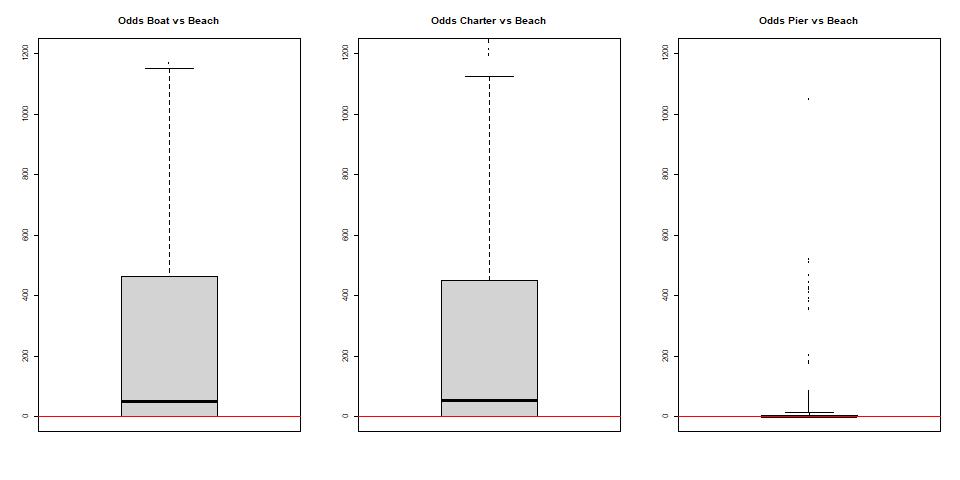
\includegraphics[scale=0.5]{Unordered Odds 1}\\

%% Model Selection
\begin{table}[H] \centering 
  \caption{Poisson Model Selection} 
  \label{} 
\resizebox{15cm}{!}{
\begin{tabular}{@{\extracolsep{5pt}}lcccccc} 
\\[-1.8ex]\hline 
\hline \\[-1.8ex] 
 & \multicolumn{6}{c}{\textit{Dependent variable:}} \\ 
\cline{2-7} 
\\[-1.8ex] & \multicolumn{6}{c}{Cards} \\ 
\\[-1.8ex] & (1) & (2) & (3) & (4) & (5) & (6)\\ 
\hline \\[-1.8ex] 
 Income & $-$0.002$^{*}$ & $-$0.002$^{*}$ & $-$0.002$^{*}$ & $-$0.002$^{*}$ & $-$0.002$^{*}$ & $-$0.002 \\ 
  & (0.001) & (0.001) & (0.001) & (0.001) & (0.001) & (0.001) \\ 
  & & & & & & \\ 
 Rating & 0.001$^{*}$ & 0.001$^{*}$ & 0.001$^{*}$ & 0.001$^{*}$ & 0.001$^{*}$ & 0.001$^{*}$ \\ 
  & (0.0003) & (0.0003) & (0.0003) & (0.0003) & (0.0003) & (0.0003) \\ 
  & & & & & & \\ 
 Age & 0.001 & 0.001 & 0.001 & 0.001 & 0.001 &  \\ 
  & (0.002) & (0.002) & (0.002) & (0.002) & (0.002) &  \\ 
  & & & & & & \\ 
 Education & $-$0.007 & $-$0.007 & $-$0.007 & $-$0.007 &  &  \\ 
  & (0.009) & (0.009) & (0.009) & (0.009) &  &  \\ 
  & & & & & & \\ 
 GenderFemale & $-$0.024 & $-$0.024 & $-$0.024 &  &  &  \\ 
  & (0.058) & (0.058) & (0.058) &  &  &  \\ 
  & & & & & & \\ 
 StudentYes & $-$0.027 & $-$0.025 & $-$0.025 &  &  &  \\ 
  & (0.100) & (0.099) & (0.099) &  &  &  \\ 
  & & & & & & \\ 
 MarriedYes & $-$0.006 & $-$0.005 &  &  &  &  \\ 
  & (0.061) & (0.060) &  &  &  &  \\ 
  & & & & & & \\ 
 EthnicityAsian & 0.015 &  &  &  &  &  \\ 
  & (0.083) &  &  &  &  &  \\ 
  & & & & & & \\ 
 EthnicityCaucasian & $-$0.003 &  &  &  &  &  \\ 
  & (0.072) &  &  &  &  &  \\ 
  & & & & & & \\ 
 Constant & 1.021$^{***}$ & 1.023$^{***}$ & 1.020$^{***}$ & 1.008$^{***}$ & 0.907$^{***}$ & 0.986$^{***}$ \\ 
  & (0.189) & (0.181) & (0.177) & (0.175) & (0.122) & (0.078) \\ 
  & & & & & & \\ 
\hline \\[-1.8ex] 
Observations & 400 & 400 & 400 & 400 & 400 & 400 \\ 
Log Likelihood & $-$697.854 & $-$697.887 & $-$697.890 & $-$698.013 & $-$698.329 & $-$698.693 \\ 
Akaike Inf. Crit. & 1,415.707 & 1,411.775 & 1,409.781 & 1,406.026 & 1,404.658 & 1,403.386 \\ 
\hline 
\hline \\[-1.8ex] 
\textit{Note:}  & \multicolumn{6}{r}{$^{*}$p$<$0.1; $^{**}$p$<$0.05; $^{***}$p$<$0.01} \\ 
\end{tabular} 
}
\end{table} 

Figure 2\\
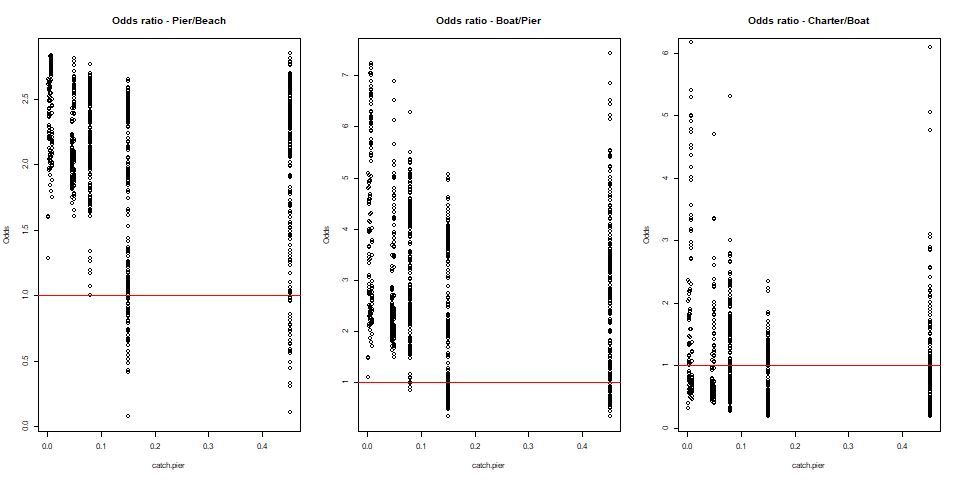
\includegraphics[scale=0.47]{Ordered Odds 3}\\
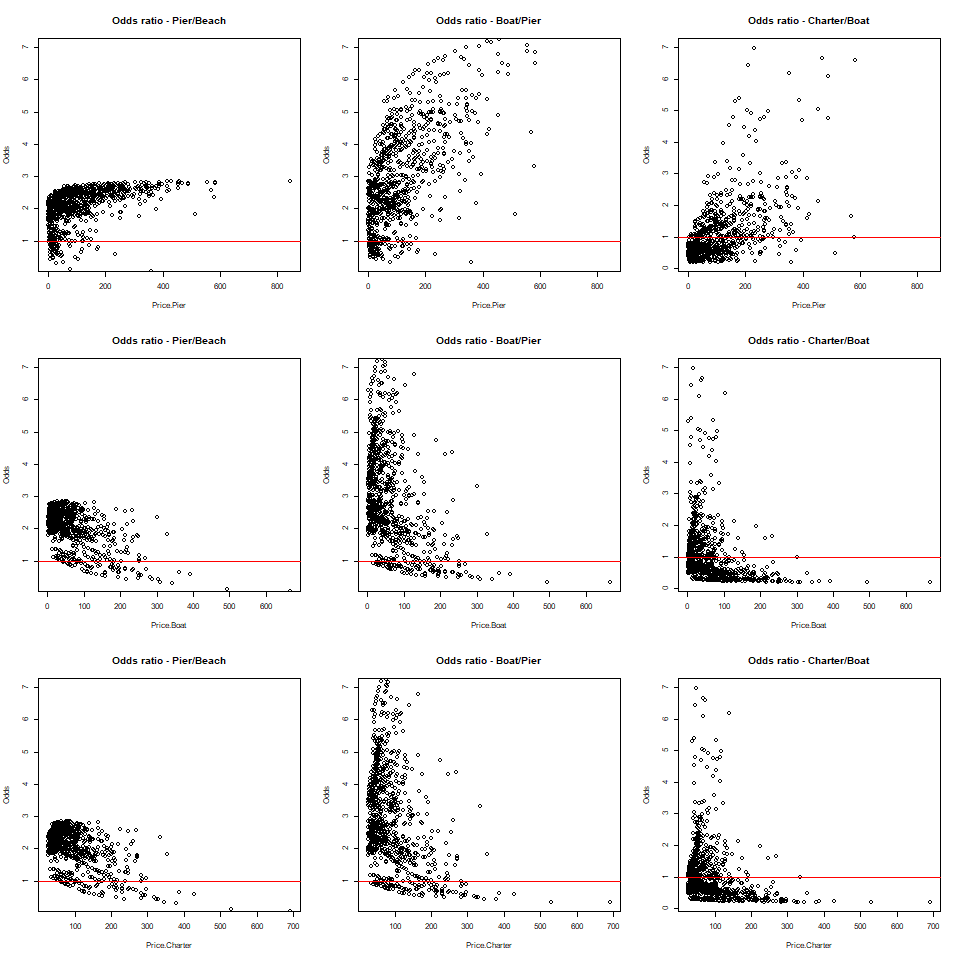
\includegraphics[scale=0.47]{Ordered Odds 2}





}
\end{document}